\section{Exemple: une toute première approche du contact avec \castem}

Dans ce chapitre, nous présentons un petit exemple simple de contact unidirectionnel sans frottement sous \castem.

\medskip
\subsection{Contact sur une surface infiniment rigide}

Dans ce premier exemple, nous proposons d'étudier un carré soumis sur sa face supérieure à un déplacement imposé et reposant, sur sa face inférieure, sur une surface infiniment rigide, comme illustré à la \fig{Fig-Cont0}.
\begin{figure}[ht]
  \center
  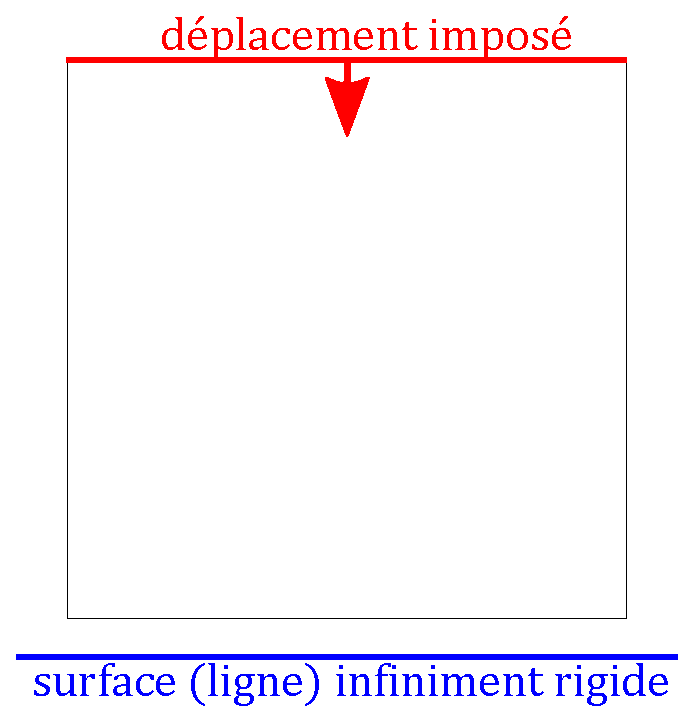
\includegraphics[height=40mm]{Contact0.eps}
  \caption{\label{Fig-Cont0} Problème de contact}
\end{figure}

\color{gris}\scriptsize
\begin{multicols}{2}
\begin{Verbatim}[numbers=left,numbersep=3pt]
OPTION ECHO 0 ;
OPTION DIME 2 ELEM QUA4 MODE PLAN CONT;
*
* Donnees
long1=10.;
nlong1=7;
uy0=-0.5;
haut1=long1;
nhaut1=nlong1;
jeu1=0.0;
*
* droite sur laquelle le carre viendra buter:
k1 = (-1.*long1) 0.;
k2 = long1 0.;
l1 = DROI (nlong1-2) k2 k1;
*
* carre:
k3 = (-0.5*long1) jeu1;
k4 = (0.5*long1) jeu1;
l2 = DROI nlong1 k3 k4;
s1 = l2 TRAN nhaut1 (0. haut1);
\end{Verbatim}
\end{multicols}
\color{black}\normalsize

\medskip
On remarquera les choses suivantes:
\begin{itemize}
  \item la ligne~$l_2$ correspondant à la face inférieure du carré «repose», sans jeu, sur la ligne~$l_1$ définissant la surface rigide sur laquelle le carré va venir buter (on aurait pu mettre un jeu initial non nul, mais ce n'est pas nécessaire);
  \item les orientations des lignes~$l_1$ et~$l_2$ sont inversées car les deux lignes en contact doivent se  «tourner le dos» au sens des normales. Cela est obligatoire;
  \item La surface de contact~$l_1$ est modélisée en utilisant~$nlong_1-2$ éléments pour le maillage, alors que le carré (ligne~$l_2$) n'en a que~$nlong_1$, afin que les maillages ne soient pas «compatibles» (i.e. que les nœuds ne tombent pas en face les uns des autres).
\end{itemize}

\color{gris}\scriptsize
\begin{multicols}{2}
\begin{Verbatim}[numbers=left,numbersep=3pt,firstnumber=last]
* Modele:
ModM1 = MODEL s1 MECANIQUE ELASTIQUE;
MatM1 = MATER ModM1 'YOUN' 1.E3 'NU' 0.3 ;
*
* CL en deplacements (Rigidites):
* 1) il faut une condition selon UX: 
*        on prend le point (0,0)
k5 = s1 POIN PROC (0. jeu1);
CLk5 = BLOQ k5 UX;
* 2) ligne de contact: rigidites
Depl1 Rigid1 = IMPO l2 l1;
Rigid2 = BLOQ DEPL l1;
* 2) ligne sur laquelle on va imposer le deplacement
l3 = s1 'COTE' 3;
CLl3 = BLOQ l3 UY ;
DCLl3 = DEPI CLl3 UY0;
* Totalite des conditions aux limites
CL0 = CLk5 ET CLl3 ET Rigid1 ET Rigid2;
\end{Verbatim}
\end{multicols}
\color{black}\normalsize

\medskip
Nous sommes en élasticité linéaire... forces et déplacements sont proportionnels et il n'y a aucun problème de convergence.

La résolution se fait le plus simplement du monde.

\color{gris}\scriptsize
\begin{Verbatim}[numbers=left,numbersep=3pt,firstnumber=last]
* RESOLUTION
MR1=RIGID ModM1 MatM1;
dep1 = RESO (MR1 ET CL0) DCLl3;
\end{Verbatim}
\color{black}\normalsize

\medskip
Puis on fait un peu d'affichage des résultats... ce qui est ilustré \fig{Fig-Cont1}.

\color{gris}\scriptsize
\begin{multicols}{2}
\begin{Verbatim}[numbers=left,numbersep=3pt,firstnumber=last]
* Post-Traitement
*
* deformee:
defo0 = DEFO (s1 ET l1) dep1 0. 'BLEU' ;
defo1 = DEFO (s1 ET l1) dep1 1. 'ROUG' ;
TITR 'Maillages non deforme (bleu) et deforme (rouge)' ;
TRAC (defo0 ET defo1) ;
*
* Deplacement selon Uy
TITR 'Champ de deplacements.' ;
DeplY1 = EXCO Dep1 UY;
TRAC DeplY1 s1;
*TRAC DeplY1 defo1;
*
* Contraintes:
Sig1 = SIGM ModM1 MatM1 Dep1;
TITR 'Champ de contraintes' ;
TRAC sig1 ModM1;
*
fin;
\end{Verbatim}
\end{multicols}
\color{black}\normalsize

\medskip
On pourra ensuite mettre~$jeu_1$ a une valeur différente de zéro et refaire le calcul. On s'apercevra que cela fonctionne toujours. La visualisation de la déformée permettra de bien comprendre comment s'effectue le calcul (on rappelle que dans \castem, toutes les conditions aux limites sont introduites par l'intermédiaire de multiplicateurs de Lagrange: voir paragraphe~\ref{Sec-cast}).

\begin{figure}[ht]
  \subfloat[déformée]{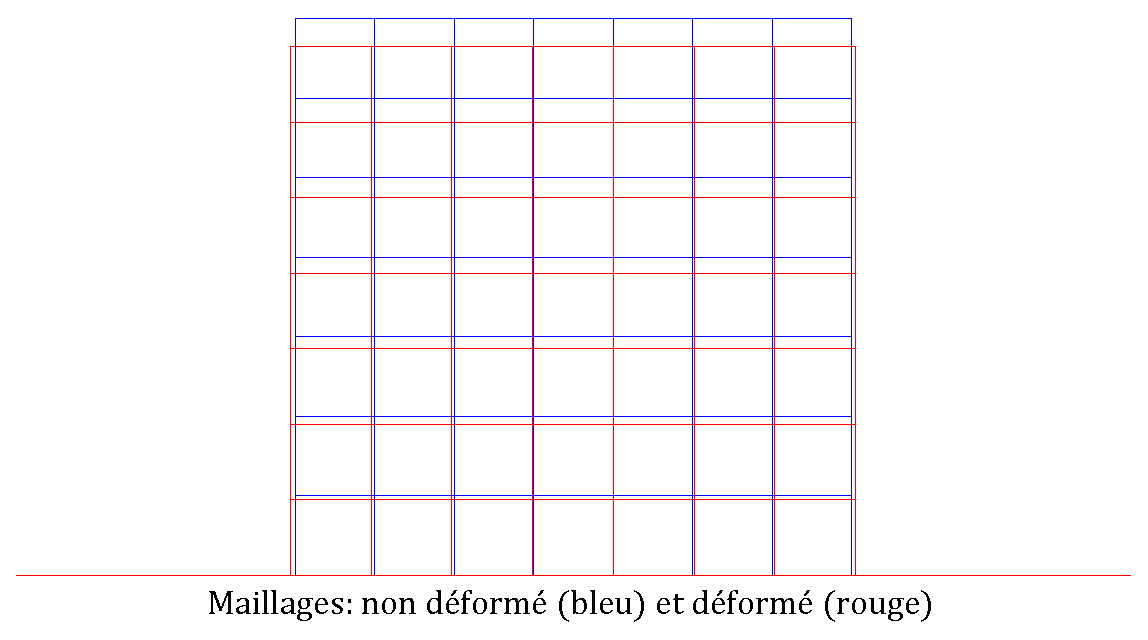
\includegraphics[height=40mm]{Contact1-def.eps}} \hfill
%  \subfloat[déplacement~$u_y$]{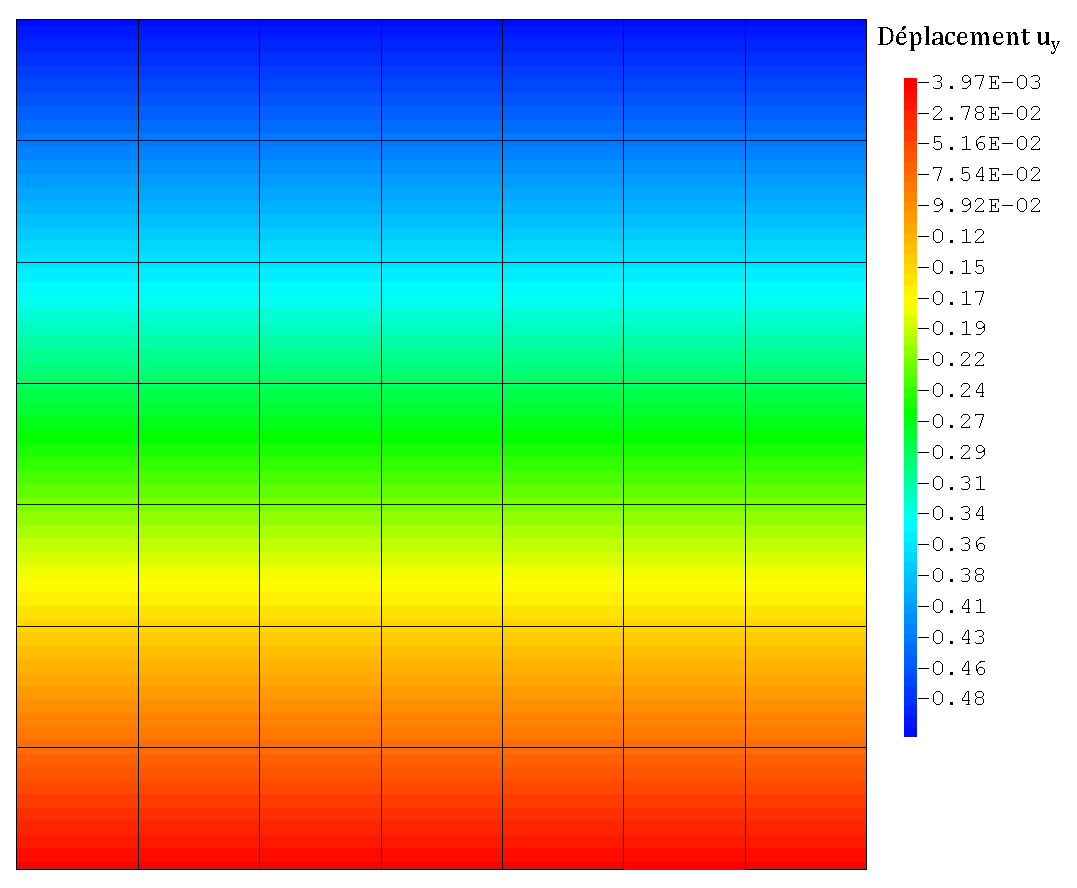
\includegraphics[height=40mm]{Contact1-uy.eps}}\hfill 
  \subfloat[forces de réactions]{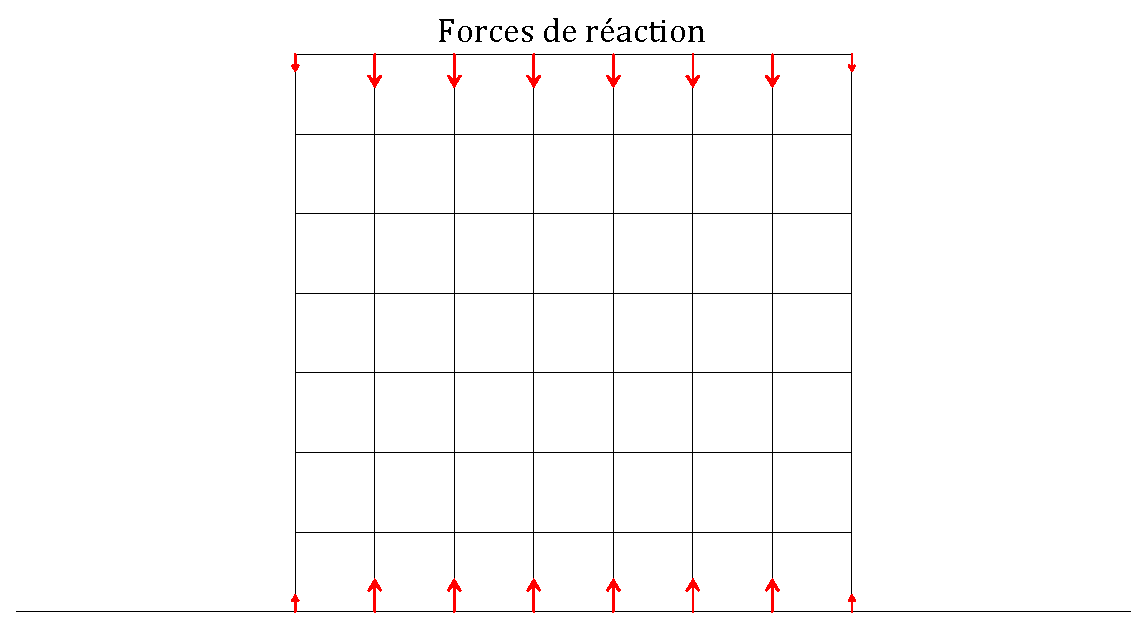
\includegraphics[height=40mm]{Contact1-reac.eps}}
  \caption{\label{Fig-Cont1} Premiers résultats sur le contact}
\end{figure}






\medskip
\subsection{Contact entre deux solides}

On peut faire une remarque sur le calcul précédent: que se passe-t-il si la surface sur laquelle on s'appuie n'est plus infiniment rigide ?

\medskip
On pourrait modéliser la partie inférieure et lui appliquer les forces de réactions qui ont été calculées précédemment.
Nous n'allons évidemment pas procéder ainsi et laisser \castem tout calculer pour nous...

\color{gris}\scriptsize
\begin{multicols}{2}
\begin{Verbatim}[numbers=left,numbersep=3pt]
OPTION ECHO 0 ;
OPTION DIME 2 ELEM QUA4 MODE PLAN CONT;
*
* Donnees
long1=10.;
nlong1=7;
uy0=-0.5;
haut1=long1;
nhaut1=nlong1;
jeu1=1.0;
*
* pave sur lequel le carre viendra buter:
k1 = (-1.*long1) 0.;
k2 = long1 0.;
l1 = DROI (2*nlong1-1) k2 k1;
s2 = l1 TRAN nhaut1 (0. (-1.0*haut1));
*
* carre
k3 = (-0.5*long1) jeu1;
k4 = (0.5*long1) jeu1;
l2 = DROI nlong1 k3 k4;
s1 = l2 TRAN nhaut1 (0. haut1);
trac (s1 et s2);
*
* Modele
ModM1 = MODEL s1 MECANIQUE ELASTIQUE;
MatM1 = MATER ModM1 'YOUN' 1.E3 'NU' 0.3 ;
ModM2 = MODEL s2 MECANIQUE ELASTIQUE;
MatM2 = MATER ModM2 'YOUN' 5.E3 'NU' 0.3 ;
*
* CL (Rigidites)
* 1) il faut une condition selon UX
k5 = s1 POIN PROC (0. jeu1);
CLk5 = BLOQ k5 UX;
* 2) ligne sur laquelle on impose le deplacement
l3 = s1 'COTE' 3;
CLl3 = BLOQ l3 UY ;
DCLl3  = DEPI CLl3 UY0;
* 3) encastrement sous la partie basse
l4 = s2 'COTE' 3;
CLl4 = BLOQ L4 DEPL;
* Totalite des conditions aux limites
CL0 = CLk5 ET CLl3 ET CLl4;
*
* RESOLUTION
Depl1 Rigid1 = IMPO l2 l1;
MR1=RIGID ModM1 MatM1;
MR2=RIGID ModM2 MatM2;
dep1 = RESO (MR1 ET MR2 ET CL0 ET Rigid1) DCLl3;
*
* Post-Traitement
*
* deformee:
defo0 = DEFO (s1 ET s2) dep1 0. 'BLEU' ;
defo1 = DEFO (s1 ET s2) dep1 1. 'ROUG' ;
TITR 'Maillages non deforme (bleu) et deforme (rouge)' ;
TRAC (defo0 ET defo1) ;
*
TITR 'Champ de deplacements.' ;
DeplY1 = EXCO Dep1 UY;
TRAC DeplY1 (s1 et s2);
*
* Comparaison des champs de contraintes:
Sig1 = SIGM (ModM1 ET ModM2) (MatM1 ET MatM2) Dep1;
TITR 'Champ de contraintes.' ;
TRAC sig1 (ModM1 ET ModM2);
*
fin;
\end{Verbatim}
\end{multicols}
\color{black}\normalsize

\medskip
Cette fois-ci, nous avons mis~$jeu_1$ a une valeur non nulle pour bien comprendre comment se fait la résolution de ce système numérique.

On obtient les résultats illustrés à la \fig{Fig-Cont21} pour la déformée et les forces de réactions et à la \fig{Fig-Cont22} pour les déplacements et contraintes.

\begin{figure}[ht]
  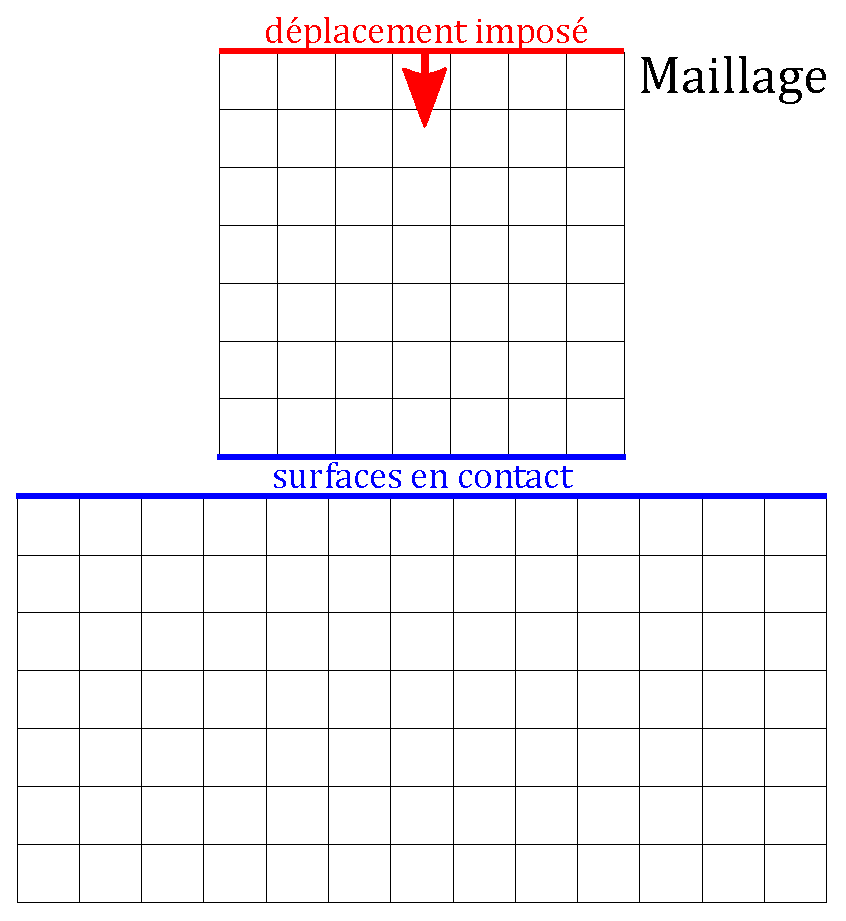
\includegraphics[height=40mm]{Contact2-pb.eps} \hfill 
  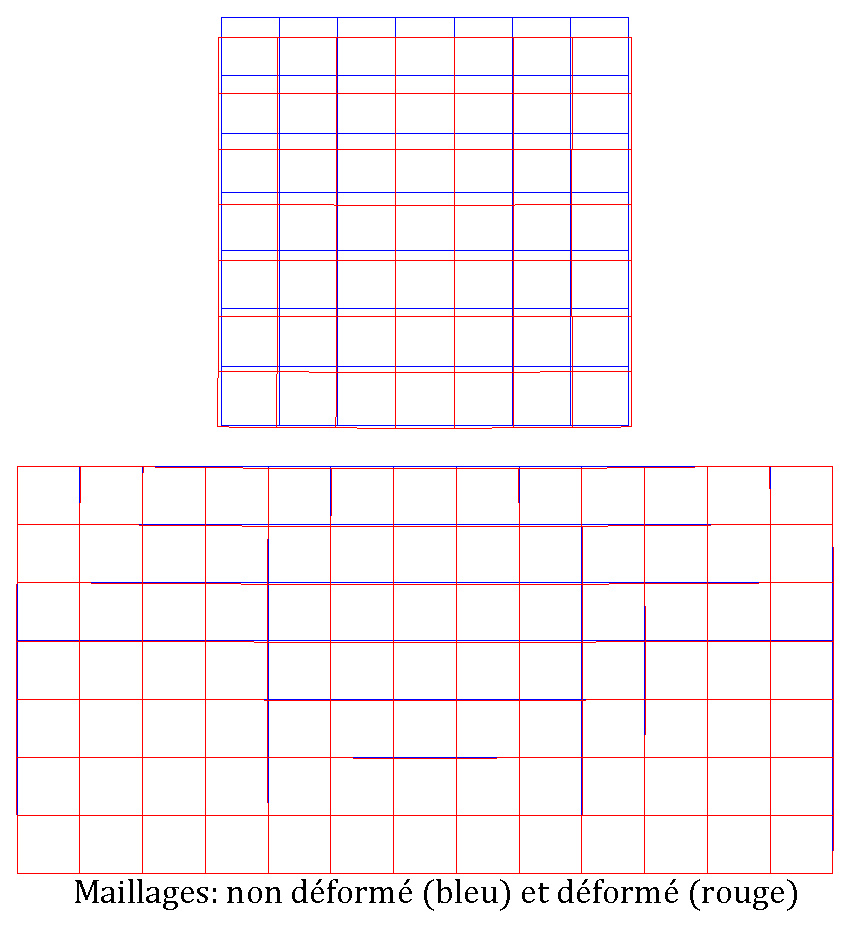
\includegraphics[height=40mm]{Contact2-def.eps}\hfill 
  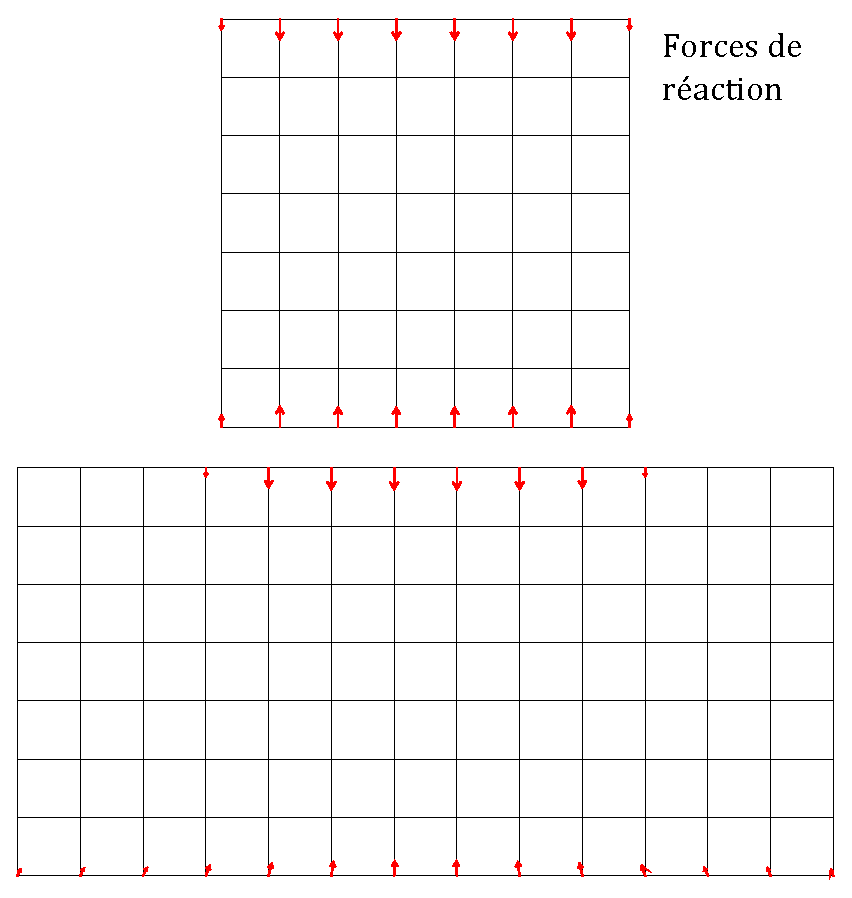
\includegraphics[height=40mm]{Contact2-reac.eps}
  \caption{\label{Fig-Cont21} a) maillage, b) déformée c) forces de réaction}
\end{figure}

\begin{figure}[ht]
  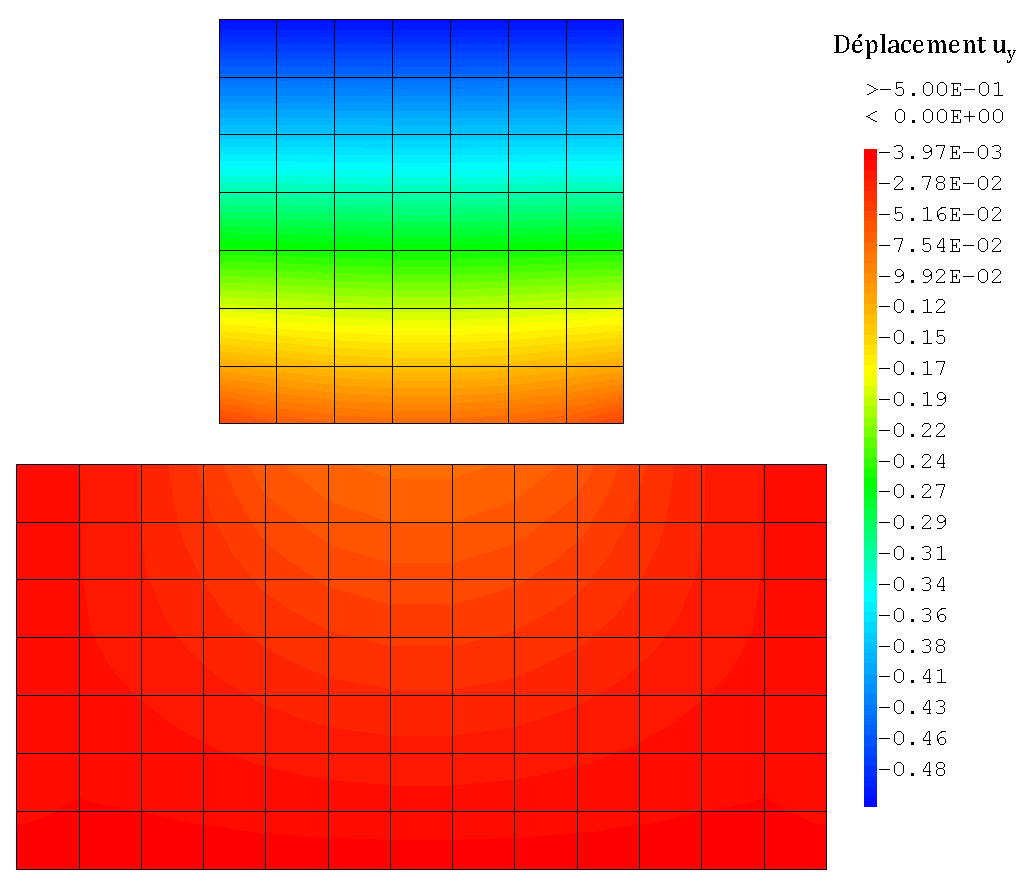
\includegraphics[height=40mm]{Contact2-uy.eps} \hfill 
  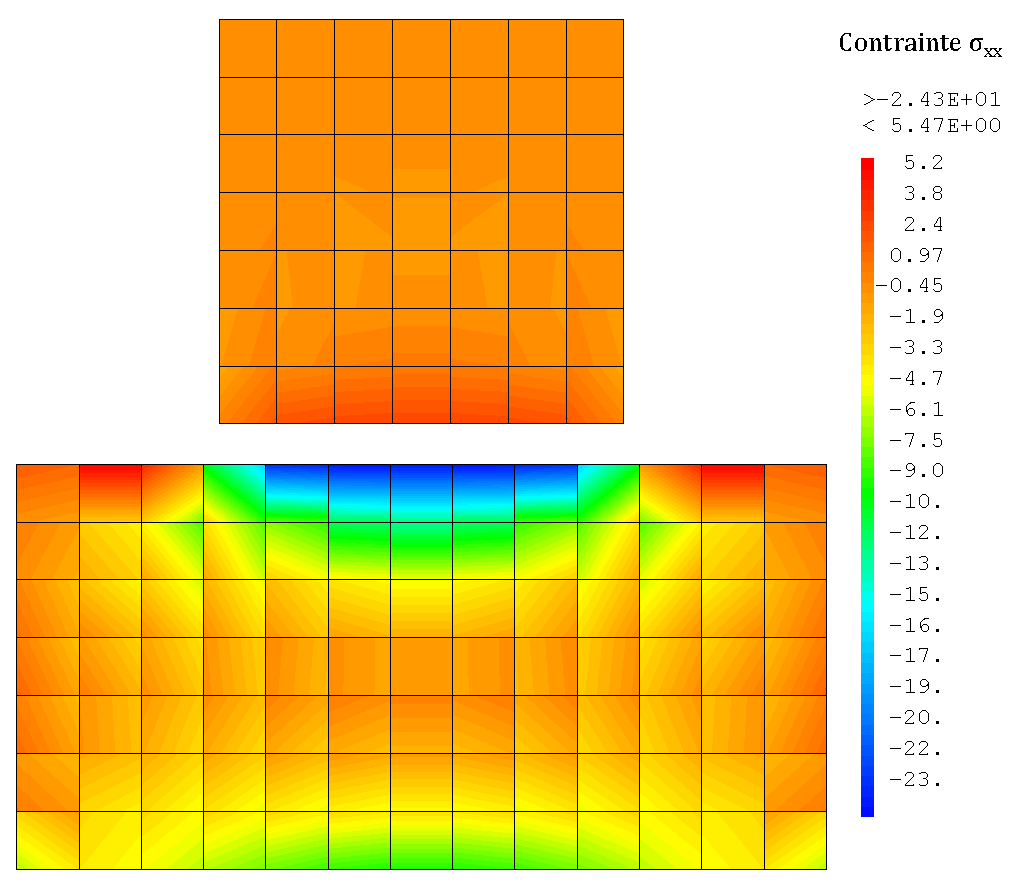
\includegraphics[height=40mm]{Contact2-sxx.eps}\hfill 
  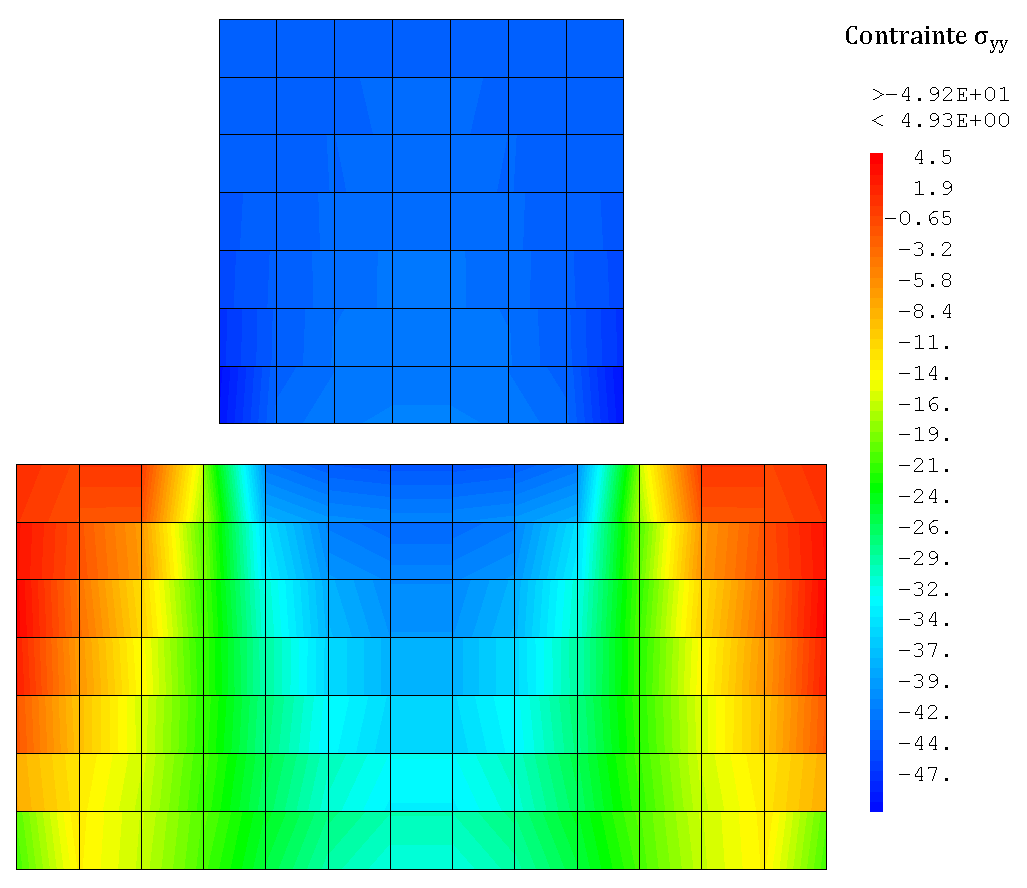
\includegraphics[height=40mm]{Contact2-syy.eps}
  \caption{\label{Fig-Cont22} a) déplacement~$u_y$ b)~$\sigma_{xx}$ et c)~$\sigma_{yy}$}
\end{figure}








\medskip
\subsection{Résolution pas à pas}

Les résolutions présentées ci-dessus étaient finalement de type classique, i.e. inversion d'un système comprenant les conditions aux limites et le chargement.

Cela fonctionnait particulièrement bien car nous étions en élasticité linéaire... mais que se passerait-il si le carré considéré avait un comportement non linéaire, en particulier s'il devait être le siège de déformations permanentes ?

On se doute aisément que le modèle rudimentaire ne fonctionnerait pas. C'est pourquoi nous allons le modifier afin d'introduire une résolution pas à pas, qui permet d'appliquer un chargement (ou un déplacement imposé) de manière progressive.

\medskip
Nous ne présentons pas ici de comportement non linéaire pour les matériaux, cela se fait en TD. Toutefois, nous présentons le même calcul que précédemment, mais codé pour une résolution pas à pas.

\medskip
Afin de définir le chargement dans le temps, nous commençons par construire la liste de réels~$Ltemp_1$ qui contient les pas de temps, à savoir~$0.0$ et~$1.0$ (2 pas de temps suffisent, puisque nous restons sur une analyse élastique linéaire dans cet exemple).

À partir de cette discrétisation du temps (vraiment sommaire pour le coup), nous définissons l'objet~$evo_1$ de type évolution pour chacun des pas de temps.~$evo_1$ est donc une fonction du temps, qui va nous servir à affecter le déplacement imposé:~$CharU_1$ est de type chargement, nécessaire pour la résolution par PASAPAS. Avec l'option DIMP, on signifie qu'il s'agit d'un déplacement imposé. Ainsi~$CharU_1$ contient l'évolution des déplacements imposés sur la condition DCLl3 au cours du temps.

\medskip
Les résultats sonr présentés à la \fig{Fig-Cont1}, après le listing.

\color{gris}\scriptsize
\begin{multicols}{2}
\begin{Verbatim}[numbers=left,numbersep=3pt]
OPTION ECHO 0 ;
OPTION DIME 2 ELEM QUA4 MODE PLAN CONT;
*
* Donnees
long1=10.;
nlong1=7;
uy0=-0.5;
haut1=long1;
nhaut1=nlong1;
jeu1=0.0;
*
* pave sur laquel le carre viendra buter:
k1 = (-1.*long1) 0.;
k2 = long1 0.;
l1 = DROI (2*nlong1-1) k2 k1;
s2 = l1 TRAN nhaut1 (0. (-1.0*haut1));
*
* carre
k3 = (-0.5*long1) jeu1;
k4 = (0.5*long1) jeu1;
l2 = DROI nlong1 k3 k4;
s1 = l2 TRAN nhaut1 (0. haut1);
trac (s1 et s2);
*
*
* Modele
ModM1 = MODEL s1 MECANIQUE ELASTIQUE;
MatM1 = MATER ModM1 'YOUN' 1.E3 'NU' 0.3 ;
ModM2 = MODEL s2 MECANIQUE ELASTIQUE;
MatM2 = MATER ModM2 'YOUN' 5.E3 'NU' 0.3 ;
*ModM1 = ModM1 ET ModM2;
*
* CL (Rigidites)
* 1) il faut une condition selon UX, on prend le point (0,0)
k5 = s1 POIN PROC (0. jeu1);
CLk5 = BLOQ k5 UX;
* 2) ligne sur laquelle on va imposer le deplacement
l3 = s1 'COTE' 3;
CLl3 = BLOQ l3 UY ;
DCLl3  = DEPI CLl3 UY0;
* 3) encastrement sous la partie basse
l4 = s2 'COTE' 3;
CLl4 = BLOQ L4 DEPL;
* 4) ligne de contact:
Depl1 Rigid1 = IMPO l2 l1;
*
* Totalite des conditions aux limites
CL0 = CLk5 ET CLl3 ET CLl4 ET Rigid1;
*
* Chargement
Ltemps1 = PROG 0. 1.;
evo1 = EVOL 'MANU' 'TEMPS' Ltemps1 (PROG 0. 1.) ;
CharU1 = CHAR DIMP DCLl3 evo1 ;
Char0 = CharU1 ;
*
* RESOLUTION
*
* Construction de la table PASAPAS:
TAB1            = TABL;
TAB1.'TEMPS_CALCULES'   = Ltemps1;
TAB1.'MODELE'       = (ModM1 ET ModM2);
TAB1.'CARACTERISTIQUES'  = (MatM1 ET MatM2);
TAB1.'BLOCAGES_MECANIQUES' = CL0;
TAB1.'CHARGEMENT'     = Char0;
*
* Resolution:
TAB2 = PASAPAS TAB1 ;
*
* Post-Traitement
*
dep1 = TAB2 . 'DEPLACEMENTS' . 1;
*
* deformee:
defo0 = DEFO (s1 ET s2) dep1 0. 'BLEU' ;
defo1 = DEFO (s1 ET s2) dep1 1. 'ROUG' ;
TITR 'Maillages non deforme (bleu) et deforme (rouge).' ;
TRAC (defo0 ET defo1) ;
*
TITR 'Champ de deplacements.' ;
DeplY1 = EXCO Dep1 UY;
TRAC DeplY1 (s1 et s2);
*
* Comparaison des champs de contraintes:
sig1 = TAB2 . 'CONTRAINTES' . 1 ;
TITR 'Champ de contraintes.' ;
TRAC sig1 (ModM1 ET ModM2);
*
* Visualisations des reactions:
reac1 = TAB2 . 'REACTIONS' . 1 ;
vr1 = VECT reac1 0.8E-2 'FX' 'FY' 'ROUG' ;
TITR 'Forces de reaction.' ;
TRAC vr1 (s1 ET s2) ;
*
fin;
\end{Verbatim}
\end{multicols}
\color{black}\normalsize

On obtient les mêmes résultats que ceux déjà présentés (voir \fig{Fig-Cont21} et \fig{Fig-Cont22}).

\bigskip
Nous pouvons mentionner également que ce type de calcul permet de calculer la géométrie de pièces réalisées en thermocompression. Considérons un matelas de matière souple placé entre le plateau supérieur d'une presse et un outil comportant un logement, comme illustré à la \fig{Fig-Thermo}a. Une fois que le plateau de presse est descendu, on obtient la pièce en forme donnée à la \fig{Fig-Thermo}b.

\begin{figure}[ht]
  \center
  \ifVersionDuDocEstVincent
     \includegraphics[width=80mm]{Thermo0.eps} \hfill
%     \includegraphics[height=40mm]{Thermo1.eps} \hfill
     \includegraphics[width=90mm]{Thermo2.eps}
  \else
     \includegraphics[width=64mm]{Thermo0.eps} \hfill
     \includegraphics[width=72mm]{Thermo2.eps}
  \fi
  \caption{\label{Fig-Thermo} Thermocompression: a) problème, b) forme de la pièce après production}
\end{figure}

\medskip
À partir des listings précédents, il est aisé d'obtenir les résultats de la \fig{Fig-Thermo}b... et nous vous invitons à le faire.

\medskip
Une fois ce premier calcul réalisé (et donc pleins de fierté et de confiance en nous), nous vous proposons d'utiliser un matelas de matière plus épais, \textcolorred{vraiment plus épais}. Le but est que lors du process, lorsque le plateau de la presse descend (situation réelle ou simulée), la matière vienne suffisamment remplir la cavité du moule pour qu'il y ait contact entre la pièce déformée et le fond de la cavité.

\bigskip
Nous allons alors constater que le contact n'est pris en compte que dans la partie supérieure du moule, mais pas sur les côtés de la cavité, ni au fond de celle-ci...

En TP, nous travaillerons à comprendre pourquoi (qu'est-ce que le code de calcul a compris de ce que nous lui avons proposé comme modélisation ?) et à réaliser un modèle correspondant à ce que nous souhaitions.
